\documentclass[a4paper, % A4
	parskip, % Absätze durch Abstand statt Einrückung gekennzeichnet
	%draft, % überlange Zeilen werden nicht%markiert
	ngerman] % english, hyphenation etc.
	{scrreprt} % Report (KOMA-Script)

\usepackage[font=small,labelfont=bf]{caption}

\usepackage[T1]{fontenc} % Font family encoding: 8 Bit
\usepackage[utf8]{inputenc} % Encoding in the created document: UTF-8
\usepackage{lmodern} % Font family
\usepackage{wrapfig}

\usepackage{csquotes}
\usepackage[babel]{microtype} % Automatische Grauwertverbesserung
\usepackage[ngerman]{babel} % warning that option english is not loaded yet
    % when not declaring [USenglish] even though documentclass sets it globally
\usepackage{IEEEtrantools} % bibliography, quoting (\cite)

\usepackage{colortbl} % Colored cells
\definecolor{grey}{RGB}{190,190,190}

\usepackage{graphicx} % include images (\includegrafics)
\usepackage[section]{placeins} % place floating objects before a \FloatBarrier

\usepackage{rotating} % used for sidewaysfigure in Projektplan
\usepackage{tabularx}

\usepackage{framed} % frame paragraphs (\begin{framed})
\usepackage{geometry} % change margin for title page (\newgeometry,
	% \resetgeometry)
\usepackage{setspace} % change line spacing (\onehalfspacing)
\usepackage{pdflscape} % pages in landscape (\begin{landscape})
\usepackage{multicol} % multiple columns for a sector (\begin{multicols})

\usepackage{booktabs} % Professional looking tables (\toprule,% \midrule,
	% \bottomrule)
\usepackage{threeparttable} % table with notes (\tnote, \begin{tablenotes})
\usepackage{longtable}

\usepackage[printonlyused, % show only used acronyms
		% withpage, % show pagenumber of first usage
	] % longform in footnote (instead of shortform)
	{acronym} % abbreviations  (\ac, \acs,\acl)
		% \begin{acronym})
		
\usepackage{pdfpages} % include PDFs (\includepdf)
\usepackage{listings} % codelistings (\lstnewenvironment)
\usepackage{float} % own floating objects (\newfloat, \floatname)

\usepackage{hyperref} % linking to refs and URLs (\ref, \url, \autoref,

% \nameref)
%rename the output for an \autoref{chap:XXX} from lowercase chapter to Chapter
% and also for Section and Subsection
\addto\extrasUSenglish{%
  \renewcommand{\chapterautorefname}{Chapter}% 
}
\addto\extrasUSenglish{%
  \renewcommand{\sectionautorefname}{Section}% 
}
\addto\extrasUSenglish{%
  \renewcommand{\subsectionautorefname}{Subsection}% 
}

\usepackage{scrhack} % \lstlistoflistings uses deprecated \float@listhead,
    % scrhack fixes this warning (redefines macros from other packages so they
    % work better with KOMAscript)

\usepackage{enumitem} %Continue enumeration
\setlist{noitemsep, topsep=0pt, parsep=0pt, partopsep=0pt, leftmargin=0pt, labelindent=0cm, labelwidth=\wd1, itemindent=*, labelsep=\dimexpr0.6cm-\wd1}

% global formatting
\onehalfspacing % 1.5x line spacing

\usepackage{color}

% colors for syntax highlighting
\definecolor{strings}{RGB}{42,0,255}
\definecolor{builtInTypes}{RGB}{127,0,85}
\definecolor{comments}{RGB}{63,127,95}

\lstdefinestyle{CPPeclipse}{
    basicstyle=\ttfamily,
    stringstyle=\color{strings},     
    keywordstyle=\color{builtInTypes} \bfseries,
    commentstyle=\color{comments},
    %emph={int,char,double,float,unsigned},
    %emphstyle={\color{blue}},
}

\definecolor{pblue}{rgb}{0.13,0.13,1}
\definecolor{pgreen}{rgb}{0,0.5,0}
\definecolor{pred}{rgb}{0.9,0,0}
\definecolor{pgrey}{rgb}{0.46,0.45,0.48}


\lstdefinestyle{JavaEclipse}{
    basicstyle=\ttfamily,
    commentstyle=\color{pgreen},
    keywordstyle=\color{pblue},
    stringstyle=\color{pred},
}

\makeatletter
\def\clearfloats {
\@@par
\ifnum\@@parshape=\z@ \let\WF@pspars\@empty \fi % reset `parshape'
\global\advance\c@WF@wrappedlines-\prevgraf \prevgraf\z@
\ifnum\c@WF@wrappedlines<\tw@ \WF@finale \fi
}
\makeatother

% Standard Listing
\lstset{
	aboveskip=1.5\baselineskip,      % space before listing
	breakatwhitespace=true,          % break only at whitespace
	breaklines=true,                 % sets automatic line breaking
	captionpos=b,                    % sets the caption-position to bottom
	extendedchars=true,              % lets you use non-ASCII characters; for 8-bits encodings only, does not work with UTF-8
	frame=single,                    % adds a frame around the code
	keepspaces=true,                 % keeps spaces in text, useful for keeping indentation of code (possibly needs columns=flexible)
	language=C++,                    % the language of the code, [11] indicates
	                                 % C++ 11syntax. other possible values:
	                                 %     ANSI, GNU, VISUAL ISO
	numbers=left,                    % where to put the line-numbers; possible values are (none, left, right)
	showspaces=false,                % show spaces everywhere adding particular underscores; it overrides 'showstringspaces'
	showstringspaces=false,          % underline spaces within strings only
	showtabs=false,                  % show tabs within strings adding particular underscores
	tabsize=3,                       % sets default tabsize in spaces
	style=CPPeclipse
}
% change the name from 'List of Listings' to something else
% \renewcommand{\lstlistlistingname}{Listingverzeichnis}
\newcommand{\code}[1]
	{\texttt{#1}}
\newcommand{\todo}[1]
    {{\color{red}<TODO:> #1}}
\newcommand{\command}[1]
    {\textit{#1}}
\newcommand{\filepath}[1]
	{\texttt{#1}}
\newcommand*{\fullref}[1]
    {\hyperref[{#1}]{\autoref*{#1} \nameref*{#1} on page \pageref*{#1}}}
\newcommand{\linenumber}[1]
    {\textit{#1}}
\newcommand{\productname}[1]
	{\textit{#1}}
\newcommand{\tbd}[1]
    {{\color{red}<tbd> #1}}
\newfloat{listingfloat}{htb}{qcl}[chapter]
\floatname{listingfloat}{Listing}

% definiton of frequenlty used standard texts.
% Usage in text: \ecdt{} -> Eclipse CDT

\newcommand{\advisor}
	{Prof. Dr. Farhad Mehta}
\newcommand{\authors}
	{Konstantin Kayed, Theodor Winter}
\newcommand{\fluxron}
    {Fluxron Solutions AG}
\newcommand{\experte}
    {Vikram Kriplaney}
\newcommand{\gegenleser}
    {Prof. Hansjörg Huser}
\newcommand{\ct}
    {class template}
\newcommand{\cts}
    {\ct{}s}
\newcommand{\ecdt}
    {\productname{Eclipse \cdt{}}}
\newcommand{\eclipse}
    {\productname{Eclipse}}
\newcommand{\ep}
    {extension point}
\newcommand{\ft}
    {function template}
\newcommand{\fts}
    {\ft{}s}
\newcommand{\pg}
    {plug-in}
\newcommand{\pgs}
    {plug-ins}
\newcommand{\place}
	{HSR---Hochschule für Technik Rapperswil \\ Institut für Software}
\newcommand{\product}
	{\productname{\ecdt{} Smartphone Applikation für intelligente, induktive Heizsysteme in Grossküchen\pg{}}}
\newcommand{\timeperiod}
	{Herbstsemester 2015}
\newcommand{\titel}
	{Smartphone Applikation für intelligente, induktive Heizsysteme in Grossküchen}
\newcommand{\viewname}
    {``Template Information View''}
\newcommand{\work}
	{Bachelorarbeit}
 
\begin{document}

%Intro-Teil
% Following the template unter www.hsr.ch > HSR-intern > Bachelor-Studiengänge
% > Informatik > allgemeine Infos Diplom-, Bachelor- und Studienarbeiten.

\newgeometry{left=2.25cm, right=2.25cm, top=2.25cm, bottom=2.25cm} % new
% margins

\begin{titlepage}

\begin{center}
\begin{minipage}[t]{0.45\textwidth}
    
\includegraphics[width=\textwidth]{start/img/hsrLogo}
\end{minipage}
\hspace{\fill} % horizontal space
\begin{minipage}[t]{0.45\textwidth}
    \vspace{-3.26cm}
    
\includegraphics[width=\textwidth]{start/img/ifsLogo} %TODO: more highres logo
\end{minipage}

\end{center}

\vspace{15ex} % vertical space
\begin{center}
	\Huge 
	\begin{framed}
		\textbf{\titel}
	\end{framed}
	
	\vspace{3ex}
	\textbf{\work}
	
	\vspace{1ex}
	\LARGE 
	\place
	
	\vspace{5ex}
	\begin{framed}
		\timeperiod
	\end{framed}
\end{center}

\vspace{11ex}
\begin{tabular}{ll} % Table
	Authoren:        & \authors    \\
	Betreuer:        & \advisor    \\
	Experte:         & \experte    \\
	Gegenleser:      & \gegenleser \\
\end{tabular}

\end{titlepage}

\restoregeometry % reset page margins

% Der Abstract richtet sich an den Spezialisten auf dem entsprechenden Gebiet
% und beschreibt daher in erster Linie die (neuen, eigenen) Ergebnisse und
% Resultate der Arbeit. Es umfasst nie mehr als eine Seite, typisch sogar nur
% etwa 200 Worte (etwa 20 Zeilen). Es sind keine Bilder zu verwenden.

\chapter*{Abstract}\addcontentsline{toc}{chapter}{Abstract}

Die Firma Fluxron Solutions AG mit Sitz in Amriswil stellt Heizlösungen und Küchengeräte auf Induktionsbasis her. Diese Geräte besitzen eine Bluetooth-Schnittstelle, über welche die Einstellungen angepasst werden können. Zudem bietet die Schnittstelle eine ausführliche Laufzeit- und Fehlerprotokollierung an. Servicetechniker benötigen genau diese Informationen zur Fehlersuche und Reparatur der Geräte in Grossküchen. Aufgrund der grossen Anzahl Geräte, ist es schwierig die Installationen im Überblick zu behalten.

In dieser Arbeit wurde eine Applikation für Android entwickelt, welche von den Technikern zur Diagnose und Konfiguration genutzt werden kann. Die Lage der verbauten Geräte wird auf Situationsfotos markiert. Damit kann bei einem Serviceeinsatz die Position und der Status aller Kochinstallationen angezeigt werden.

Zur Umsetzung des Projektes wurden agile Softwareentwicklungsmethoden eingesetzt. Neben einer gründlichen Anforderungsanalyse wurde die Benutzeroberfläche mit Mockups konzipiert und mittels Usability Walkthroughs validiert.

Als Programmiersprache wurde Java 7 für Android eingesetzt. Die Anwendungsarchitektur besteht aus drei Layern, welche mittels Messages über ein Event Bus System kommunizieren. Um eine zeitgemässe Benutzeroberfläche zu erstellen, wurde diese im schlichten aber effektiven Material Design umgesetzt. Lokal werden die Daten in einer dokumentbasierten Datenbank gespeichert. Die Kommunikation mit den Geräten erfolgt über das CANopen Protokoll. Darüber hinaus bietet die Anwendung konzeptionelle Unterstützung für eine Anbindung an ein Cloud-Backend.

Der Funktionsumfang der Mobilapplikation umfasst die Verwaltung mehrerer Küchen und der darin verbauten Geräte. Küchen können zur besseren Übersicht in einzelne Bereiche unterteilt werden. Die Geräte eines Bereichs werden regelmässig zur Statusaktualisierung abgefragt. \todo{V1 - AKTUALISIERUNG NÖTIG!}
% Das Management Summary richtet sich in der Praxis an die "Chefs des Chefs", d.
% h. an die Vorgesetzten des Auftraggebers (diese sind in der Regel keine
% Fachspezialisten).
% Die Sprache soll knapp, klar und stark untergliedert sein.
% Zu verwenden ist folgenden Gliederung:
% - Ausgangslage - Vorgehen, Technologien - Ergebnisse - Ausblick (optional)

\chapter*{Management Summary}\addcontentsline{toc}{chapter}{Management Summary}

    Todo Einleitung

\textbf{Motivation}

    Todo Motivation
    
\textbf{Ziele}

    Todo Ziele
    
\textbf{Resultate}

    Todo Resultate


%TODO: Selbststaendigkeitserklaerung als pdf unter start/erklaerung includen.
%\includepdf[pages=-, pagecommand={},
%scale=0.73, trim=80 210 80 80]{start/erklaerung}

%TODO: Index auf Deutsch
\addcontentsline{toc}{chapter}{Table of Contents}
\tableofcontents

%Hauptteil here
% Index of /analysis/

\chapter{Analyse}
\label{chap:Analyse}

% Ausgangslage (Ist-Analyse)

\section{Ausgangslage}
\label{sec:Ausgangslage}

\subsection{Anwendungsumfeld}
\label{subsec:Anwendungsumfeld}

%TODO
% Freistellen
\piccaption{Induktionsherd}
\parpic{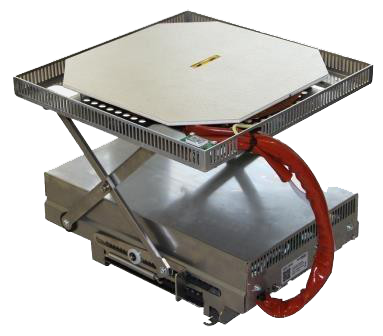
\includegraphics[scale=0.4]{analysis/res/einbaugeraete}}
Die Firma Fluxron AG mit Sitz in Amriswil TG bietet induktive Heiz- und Energiesysteme für Grossküchen an. Die Produktpalette besteht aus verschiedenen Induktionsherden und Thermostatsystemen. Diese haben jeweils ein Bluetoothmodul eingebaut, welches auf ein CANopen-basiertes Protokoll zur Kommunikation setzt. Die Module liefern neben den Geräteeinstellungen auch Fehlercodes und Sensormesswerte via Blootooth.
\picskip{0}
Fluxron verkauft diese Induktionsgeräte an Servicefirmen, welche diese dann beim Endkunden, z.B. einem Restaurant, einbauen und installieren. Dabei, aber auch bei Wartungsarbeiten, setzen die Servicefirmen die bestehende Android Applikation \enquote{FLX Tool} zur Diagnose und zur Konfiguration ein.

Neben den Servicefirmen, setzen auch die Mitarbeiter der Firma Fluxron die Androidapplikation bei internen Versuchen oder zur Ferndiagnose ein. Bei der Ferndiagnose wird eine Teamviewer-Verbindung auf das Smartphone oder den PC des Technikers aufgebaut. Über diese kann dann eine Diagnose mittels den Tools via Bluetooth erfolgen.

\subsection{Bestehende Android-Applikation - Fluxron Systemkonfigurator }
\label{subsec:Bestehende Smartphone-Applikation}
In Eigenentwicklung wurde bei Fluxron bereits eine einfache Android-Applikation entwickelt. Diese unterstützt bereits das Suchen von Geräten, sowie das Lesen und Schreiben von Parametern. Da diese App allerdings immer nur ein Gerät gleichzeitig bedienen kann und die Benutzerinteraktion daher sehr Zeitaufwändig ist, soll im Rahmen dieses Projektes eine neue, übersichtlichere Androidapplikation entstehen. In den nachfolgenden Abschnitten sind die Funktionen dieser Applikation aus funktioneller Sicht aufgelistet.

%TODO Screenshots

\subsubsection{Installation und Konfiguration}
\label{subsubsec:Installation und Konfiguration}
Die App kann ist öffentlich im Google Play Store erhältlich. Nach dem Download muss der Benutzer aber ein Kennwort eingeben, um Zugang zur App und den Gerätefunktionen zu erhalten.

\subsubsection{Verbindungsaufbau zu einem Gerät}
\label{subsubsec:Verbindungsaufbau zu einem Gerät}
Um eine Verbindung mit einem Gerät herzustellen, muss dieses zuerst über einen Suchlauf gefunden werden. Der Suchlauf zeigt alle momentan aktiven Geräte in einer Liste mit ihrer Device-ID an. In der Liste sind neben den aktiven Geräten auch alle Geräte aufgelistet, welche schon einmal mit der App verbunden waren.

Danach kann man sich mit einem Gerät aus der Liste verbinden um mit dem Gerät zu interagieren.

\subsubsection{Statusansicht}
\label{subsubsec:Statusansicht}
Wenn ein Gerät verbunden ist, kann der Benutzer über die entsprechende Schaltfläche zum Gerätetyp zu der Statusübersicht des Gerätes gelangen. Auf der Statusübersicht kann der Benutzer u.a. folgende Informationen auslesen:
\begin{itemize}
\item Statuscode
\item Temperatur des Kühlkörpers
\item Temperaturgradient
\item Pfannenerkennung
\item Soll- und Ist-Temperaturen der einzelnen Zonen
\item Leistungsaufnahme
\end{itemize}

\subsubsection{Setupansicht}
\label{subsubsec:Setupansicht}
Wenn ein Gerät verbunden ist, kann in der Setupansicht eine Liste aller Parameter des Gerätes ausgelesen werden. Der Benutzer kann Parameter anwählen, eine kurze Beschreibung dazu ansehen und deren Werte ändern.

\subsubsection{Historyansicht}
\label{subsubsec:Ansichten}
In der Historyansicht können Betriebszähler eingesehen. Dies beinhaltet Werte wie z.B. die Anzahl von "Power-On" Events oder Laufzeit des Gerätes.

Neben den Zähler kann ein Fehlerlog eingesehen werden, welches die letzten Zehn Fehlercodes beinhaltet. Dies kann zur Diagnose von Problemen sehr hilfreich sein.

\subsubsection{Einschränkungen der App}
\label{subsubsec:Einschränkungen der App}
\begin{itemize}
\item Es kann immer nur ein Gerät gleichzeitig verbunden sein
\item Für jede Verbindung ist ein erneuter Suchlauf nötig
\item Die Geräte sind nur mit der ID sichtbar, dies macht die Orientierung in einer Grossküche mit einem dutzend Geräten schwierig
\item Wenn ein nicht verbundenes Gerät eine Fehlermeldung absetzt, wird diese nicht empfangen
\item Typ der verbundenen Geräte wird zwar erkannt, die Benutzeroberfläche bietet aber immer noch alle Gerätetypen an
\end{itemize}

\subsection{Weitere bestehende Software}
\label{subsec:Weitere bestehende Software}
\subsubsection{FLX Access}
\label{subsubsec:FLX Access}
\piccaption{FLX Access}
\parpic{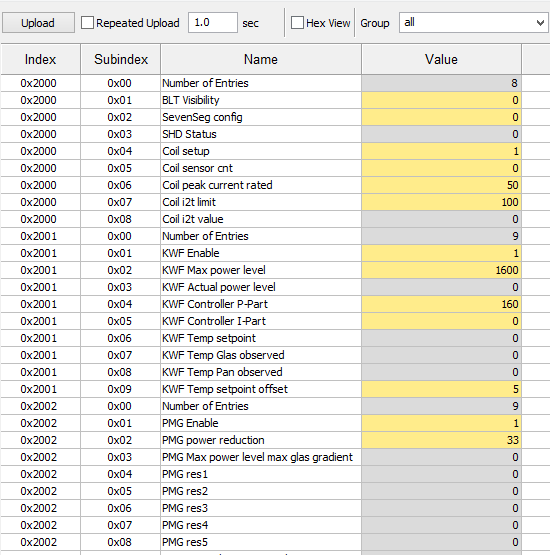
\includegraphics[scale=0.4]{analysis/res/flxaccess}}
Mit FLX Access stellt Fluxron ein Windows-Tool zum auslesen und setzen von gerätespezifischen Parametern bereit. Die Kommunikation erfolgt via Bluetooth. Zudem kann der Gerätestatus ausgelesen werden. 

Dieses System ist besonders für die Entwicklungsphase von Geräten gedacht.
\picskip{0}
\subsubsection{FLX Downloadtool}
\label{subsubsec:FLX Downloadtool}

\piccaption{FLX Access}
\parpic{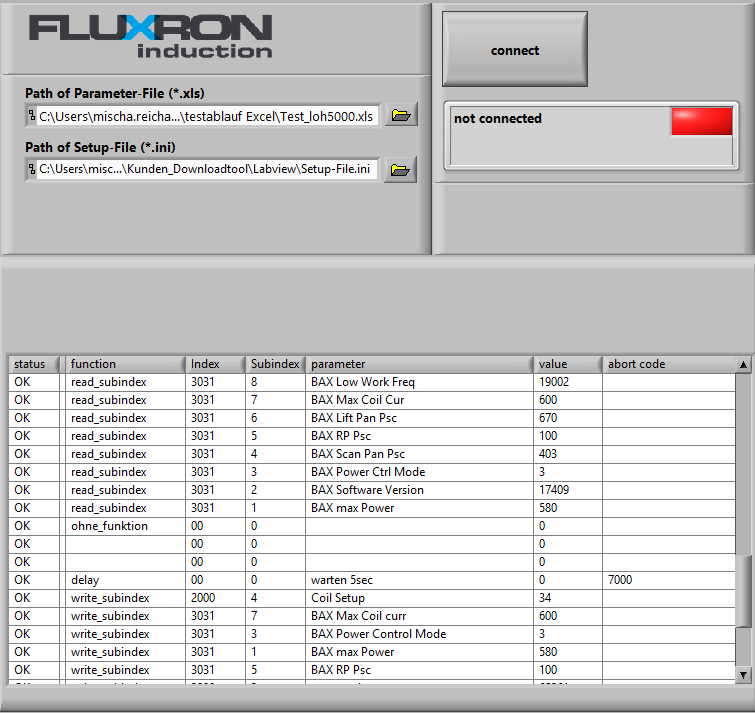
\includegraphics[scale=0.25]{analysis/res/flxdltool}}
Das FLX Downloadtool ermöglicht den Download der gesamten Konfiguration in eine Excel-Datei. In dieser können dan die Parameter eingestellt werden. Danach werden die Einstellungen über das Tool wieder auf das Gerät geladen.

Eingesetzt wird dieses Programm für das Schreiben von kundenspezifischen Parametern auf mehrere Geräte.
\picskip{0}

% NFR

\section{Non Functional Requirements}
\label{sec:Non Functional Requirements}

\begin{itemize}
\item Die Applikation soll 30 - 50 Fluxron Geräte problemlos verwalten können. In einzelnen Spezialfällen kann es aber bis zu 150 Geräte geben. Die App sollte damit ebenfalls umgehen können, allerdigs sind leichte Einschränkungen kein Problem.
\item Die Applikation soll modular aufgebaut sein, so dass zukünftige Erweiterungen leicht realisiert werden können.
\item Der Code soll so dokumentiert werden dass eine Weiterentwicklung der Applikation durch die FLUXRON Solutions AG möglich ist.
\item Die Applikation soll auf Android Geräten die bis zu 2 Jahre alt sind lauffähig sein.
\item Sowohl Bluetooth Classic als auch Bluetooth 4.0 sollen von der Applikation unterstützt werden.
\item Die Applikation soll so einfach bedienbar sein dass keine Schulung der Benutzer erforderlich ist.
\item Die Applikation soll auch ohne bestehende Internet-Verbindung vollständig funktionsfähig sein.
\end{itemize}


\subsection{Anforderungen an Android-Version}
\label{subsec:Non Functional Requirements}
Aufgrund der alten Produktgeneration muss die App auf einer Android-Version laufen, welche klassische Bluetoothverbindungen unterstützt. Zudem sollte die App auch auf einer neuen Version von Android mit Bluetooth 4.0 \ac{LE} betrieben werden können.

Bluetooth 4.0 unterstützt sowohl klassische Bluetoothverbindungen, als auch die neuen Low Energy Verbindungen. Die klassichen Verbindungen sind rückwärtskompatibel mit den Vorgängerwersionen.\cite{bt_standard}

Android unterstützt Bluetooth 4.0 (inklusive \ac{LE}) ab der API-Version 4.3\cite{bt_android}. Dies ist somit die minimal nötige Version, um die Kompatibilität zu gewährleisten.

Mit der Auswahl der Version 4.3 (Android JellyBean) können somit mehr als 50\% der momentan im Umlauf \cite{android_distribution} befindlichen Geräte unterstützt werden.
% Index of /projectmanagement/

\chapter{Projektmanagement}
\label{chap:Projektmanagement}

% Risikomanagement

\section{Risikomanagement}
\label{sec:Risikomanagement}

\begin{table}[H]
\begin{tabularx}{\textwidth}{l|>{\raggedright\arraybackslash}X}
\multicolumn{2}{l}{\textbf{R1: Erwartungen des Kunden nicht erfüllt }} \\
\hline
Beschreibung & Die Applikation erfüllt die funktionalen oder gestalterischen Erwartungen des Kunden nicht.\\
\hline
Massnahme & Es wird mit dem Kunden eine wöchentliche Besprechungen per Skype durchgeführt. Dabei wird der aktuelle Stand der Arbeit gezeigt.\\
\hline
Vorgehen beim Eintreffen & Applikation gemäss den Wünschen des Kunden anpassen.
\\
\end{tabularx}
\caption{Risiko - Erwartungen des Kunden nicht erfüllt}
\end{table}

\begin{table}[H]
\begin{tabularx}{\textwidth}{l|>{\raggedright\arraybackslash}X}
\multicolumn{2}{l}{\textbf{R2: Performance reicht nicht für das Verwalten von 100 Geräten }} \\
\hline
Beschreibung & Die Performance der Applikation reicht nicht aus um 100 Fluxron Geräte pro Küche zu verwalten beziehungsweise grafisch darzustellen.\\
\hline
Massnahme & Bei der Entwicklung werden Performance Tests mit bis zu 100 simulierten Fluxron Geräten durchgeführt.\\
\hline
Vorgehen beim Eintreffen & Die maximale Zahl von Geräten pro Küche reduzieren.
\\
\end{tabularx}
\caption{Risiko - Performance reicht nicht}
\end{table}

\begin{table}[H]
\begin{tabularx}{\textwidth}{l|>{\raggedright\arraybackslash}X}
\multicolumn{2}{l}{\textbf{R3: Bluetooth Classic und 4.0 nicht in der gleichen Applikation }} \\
\hline
Beschreibung & Es ist nicht möglich Unterstützung für Bluetooth Classic und 4.0 in der gleichen Applikation anzubieten.\\
\hline
Massnahme & In der Inception Phase wird die Bluetooth Unterstützung von Android recherchiert. Es wird nach Möglichkeit eine Android Version gewählt die beide Bluetooth Standards unterstützt.\\
\hline
Vorgehen beim Eintreffen & Es wird nur Unterstützung für Bluetooth Classic angeboten.
\\
\end{tabularx}
\caption{Risiko - Bluetooth Classic \& 4.0 Unterstützung}
\end{table}

% Meilensteine

\section{Meilensteine}
\label{sec:Meilensteine}


\begin{table}[H]
\begin{tabularx}{\textwidth}{ c | l | X | l}
\textbf{MS} & \textbf{Name} & \textbf{Resultate}  & \textbf{Datum} \\ \hline
MS1 & Kickoff              & Aufgabenstellung & 09.09.2015 \\ \hline
MS2 & Ende Inception       & Infrastruktur, Ausgangslage, Anforderungsspezifikation, Projektplan, Risikomanagement, Use Cases, Testspezifikation, Domainanalyse, Arbeitspakete	& 29.09.2015 \\ \hline
MS3 & Architekturprototyp  & Prototyp	& 13.10.2015 \\ \hline
MS4 & Zwischenpräsentation & Kunde und Experte informiert & 26-31.10.2015 \\ \hline
MS5 & Feature 75\%         & 75\% aller Features erarbeitet & 10.11.2015 \\ \hline
MS6 & Produkt fertig       & Alle geforderten Funktionen der Applikation sind implementiert. & 22.11.2015 \\ \hline
MS7 & Ende Testphase       & Testprotokolle sind vorhanden & 06.12.2015 \\ \hline
MS7 & Abgabe Abstract      & Das Abstract wurde an den Betreuer abgegeben. & 10.12.2015 \\ \hline
MS8 & Abgabe Bericht       & Der Bericht wurde an den Betreuer abgegeben. & 18.12.2015 \\
\end{tabularx}
\caption{Meilensteine}
\end{table}

% Projektplan

\clearpage
\begin{sidewaysfigure}
\section{Projektplan}
\label{sec:Projektplan}
\centering
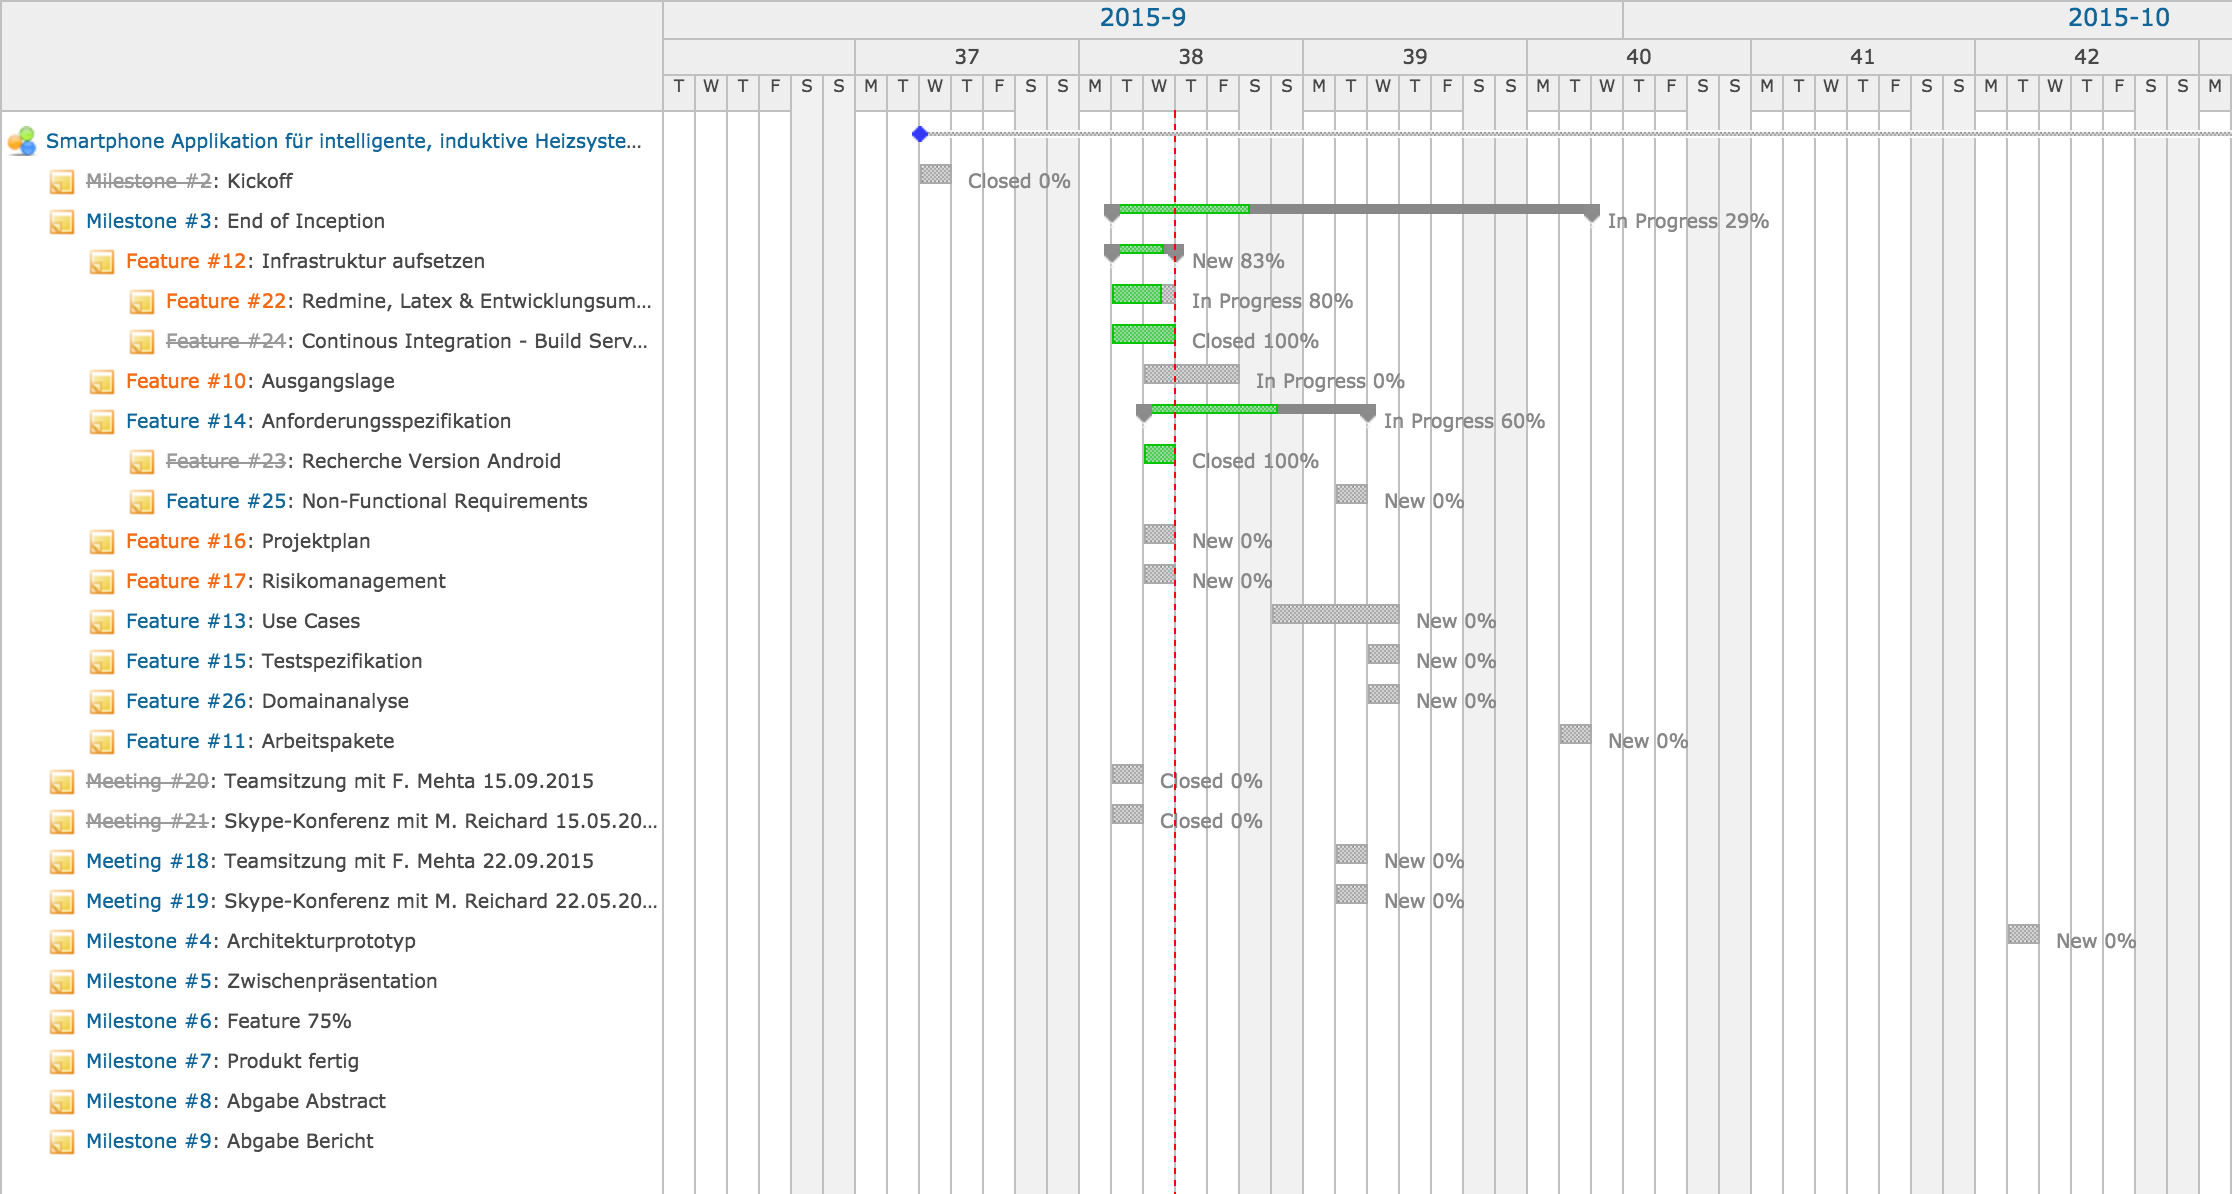
\includegraphics[scale=0.45]{projectmanagement/res/projektplan.png}
\end{sidewaysfigure}
\clearpage
% Index of /design/

\chapter{Konzeption und Design}
\label{chap:Konzeption und Design}

\section{Code Style Guidelines}
\label{sec:Code Style Guidelines}

Um die Zusammenarbeit mit mehreren Personen zu regeln, verwenden wir den folgende Code Style Guide: \url{https://source.android.com/source/code-style.html#java-language-rules}.

Zur Vereinfachung einer späteren Veröffentlichung achten wir von Anfang an auf die Android Launch Checkliste:\\ \url{http://developer.android.com/distribute/tools/launch-checklist.html}.

\subsection{Einschränkungen}
Die folgenden Empfehlungen aus dem Code Style Guide werden wir nicht übernehmen:

\begin{itemize}
\item \textbf{Jedes File hat zuoberst ein Copyright Statement.} \\ Der gesamte Code erhält eine Lizenz welche zentral abgelegt wird. Bei jedem File ein solches Statement einzufügen ist unnötig und wäre redundant.
\item \textbf{Statische Variablen beginnen mit s. Nicht-öffentliche, nicht-statische Variablen beginne mit m. Alle andern werden klein geschrieben.} \\ Diese Konvention ist unnötig da man diese Informationen problemlos auch dem Code entnehmen kann. Moderne IDEs wie Android Studio unterstützen einem dabei zusätzlich durch farbliches Hervorheben. In diesem Projekt werden alle Variablen, ausser Konstanten, klein geschrieben. Konstanten werden vollständig aus Grossbuchstaben zusammengesetzt.
\end{itemize}

\section{UX Guidelines}
\label{sec:UX Guidelines}

Bei der Entwicklung des User Interfaces nutzen wir den Material Design Style Guide:
\url{https://developer.android.com/design/index.html}. Dieser Guide ist eigentlich für Android 5.0 ausgelegt, unsere Applikation muss jedoch von Android 4.3 an lauffähig sein. Daher müssen einige Einschränkungen, z.B. bei der Verwendung von Animationen, in Kauf genommen werden.


\section{Architektur}
\label{sec:Architektur}

\subsection{Rahmenbedingungen}
\begin{figure}[H]
    \begin{center}
    		% GFX Trim left bottom right top
        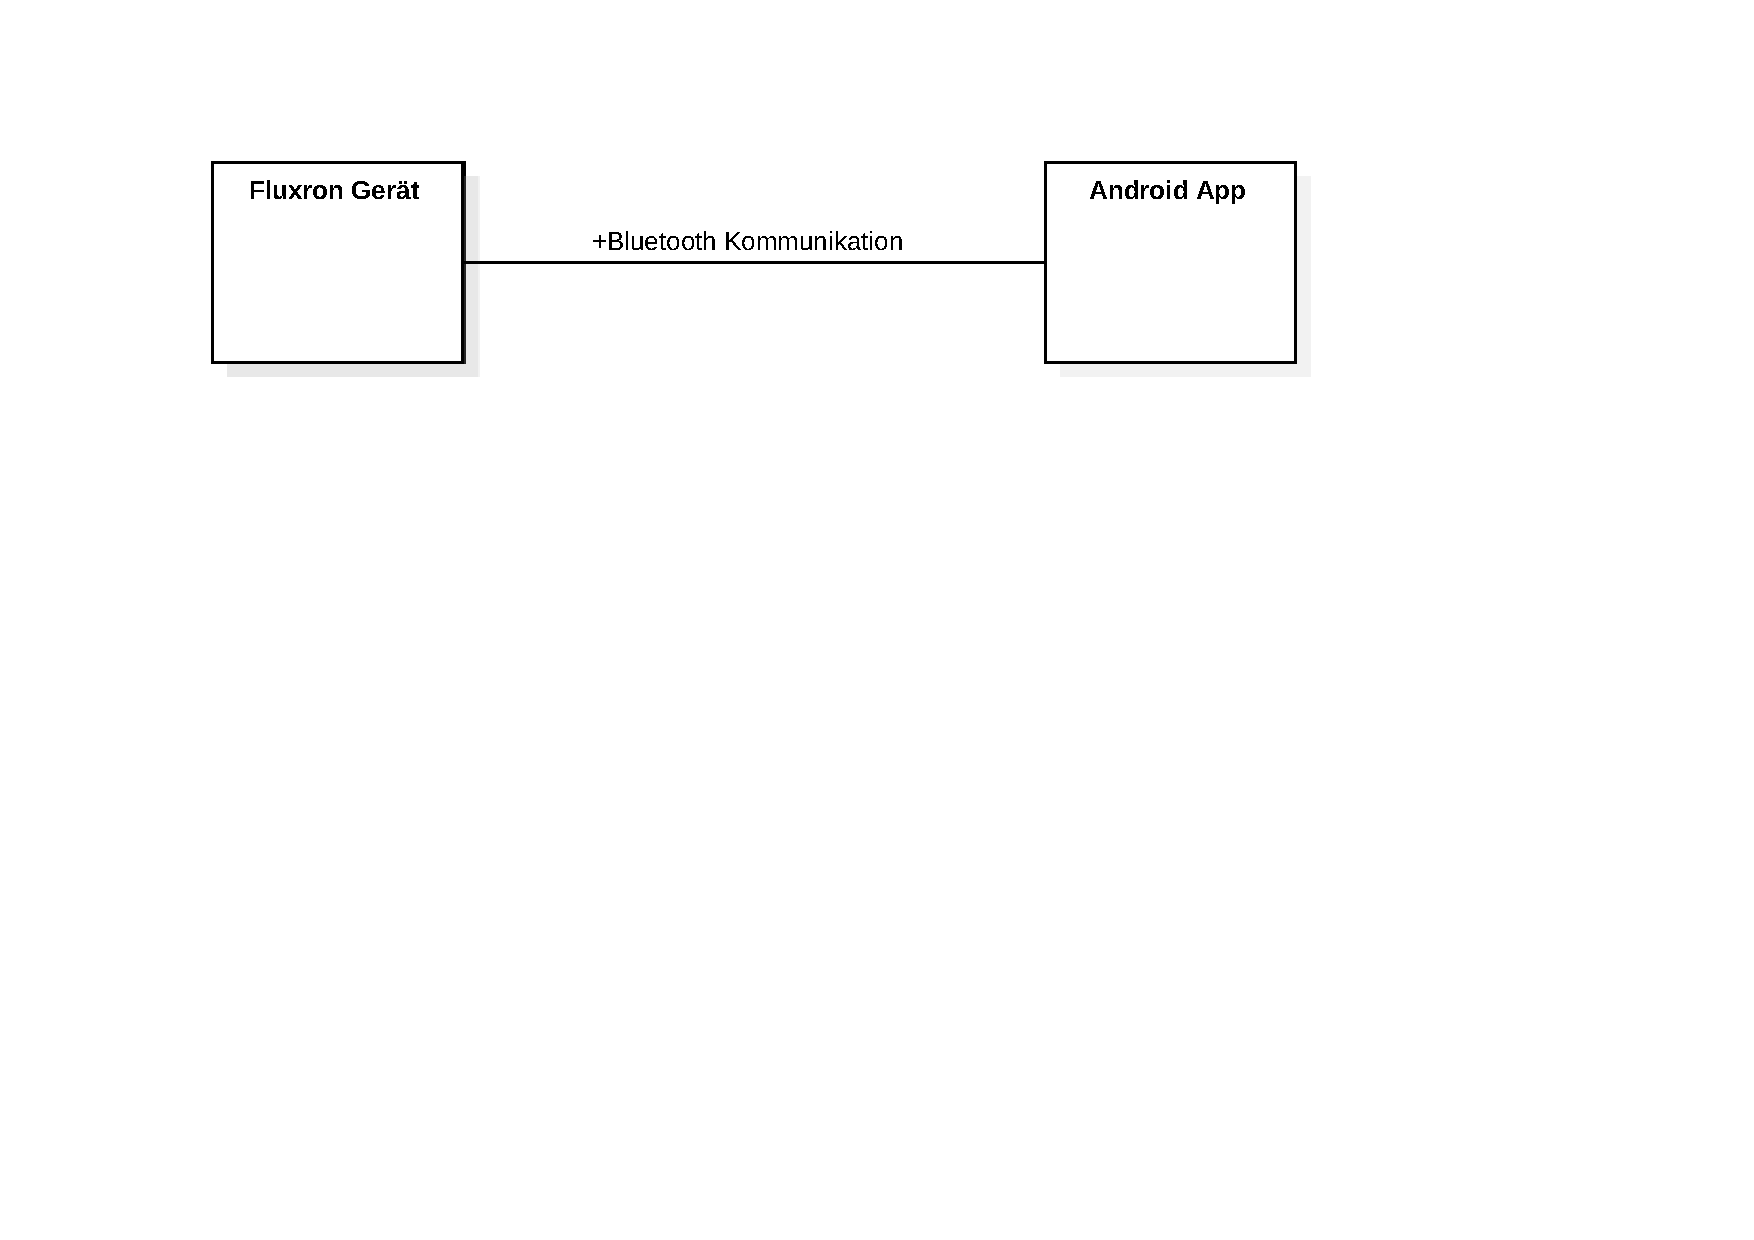
\includegraphics[trim=30 420 140 60,clip,width=\textwidth]{design/res/blackbox}
    \end{center}
    \caption{Blackbox Darstellung}
\end{figure}

Die Applikation kommuniziert mit bis zu 150 Fluxron Geräten via Bluetooth. Auf Grund der Natur von Bluetooth Geräten ist mit einer stark asynchronen Kommunikation zu rechnen. Die Architektur der Fluxron Geräte ist bereits vorgegeben. Die Kommunikation  zwischen den Geräten und der Applikation basiert auf CANopen.

Es soll eine Weiterentwicklung der Applikation durch die \fluxron{} möglich sein.

Die konzeptionellen Anforderungen der \ac{FR}15-18 sowie \ac{NFR}2, 3 sollen durch die Architektur unterstützt werden.

\subsection{Variante A: Schichtenarchitektur}
\begin{figure}[H]
    \begin{center}
    		% GFX Trim left bottom right top
        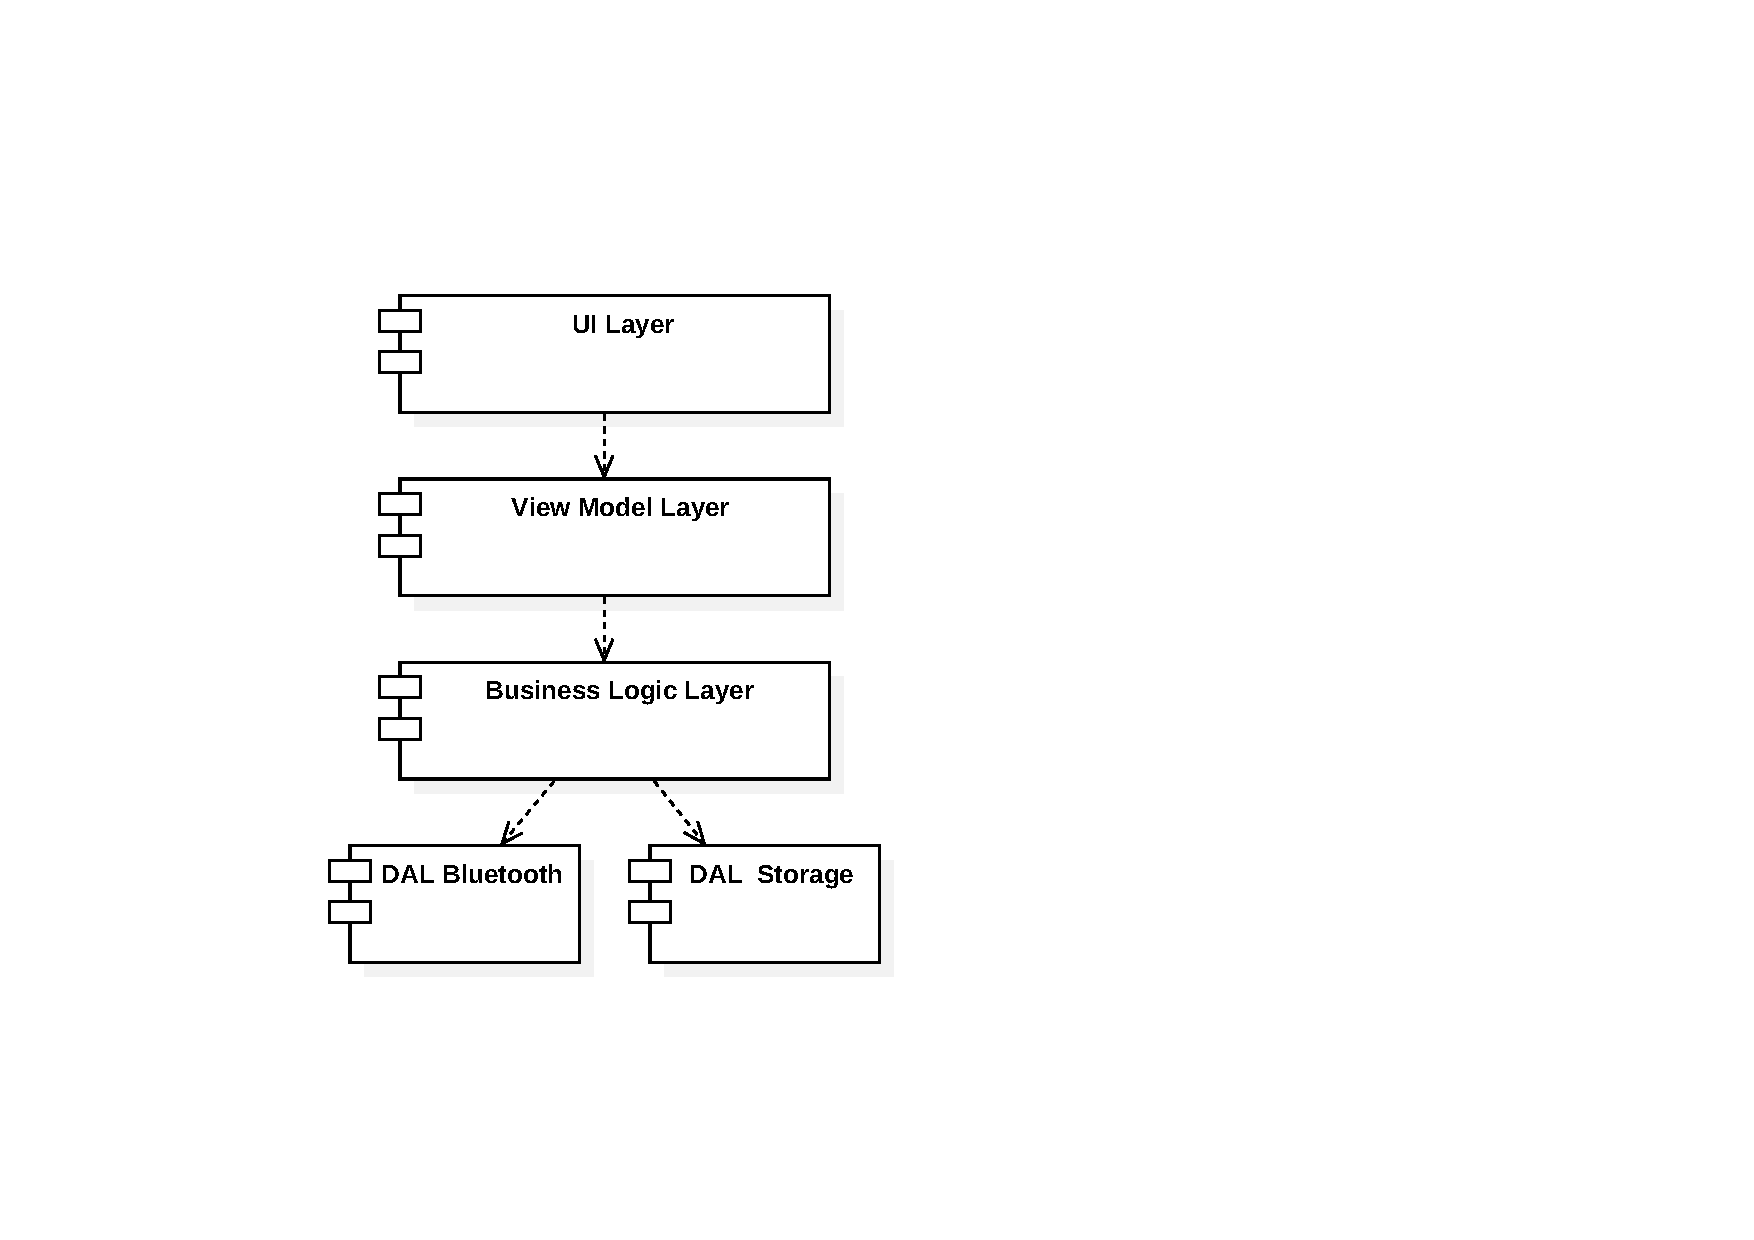
\includegraphics[trim=-100 130 140 110,clip,width=\textwidth]{design/res/layers}
    \end{center}
    \caption{Layer Architektur}
\end{figure}

Die Architektur wird in mehrere Schichten unterteilt. Dabei wird die Kopplung in die Gegenrichtung durch Interfaces und Observer aufgelöst.

\subsection{Variante B: MVC Architektur}
\begin{figure}[H]
    \begin{center}
    		% GFX Trim left bottom right top
        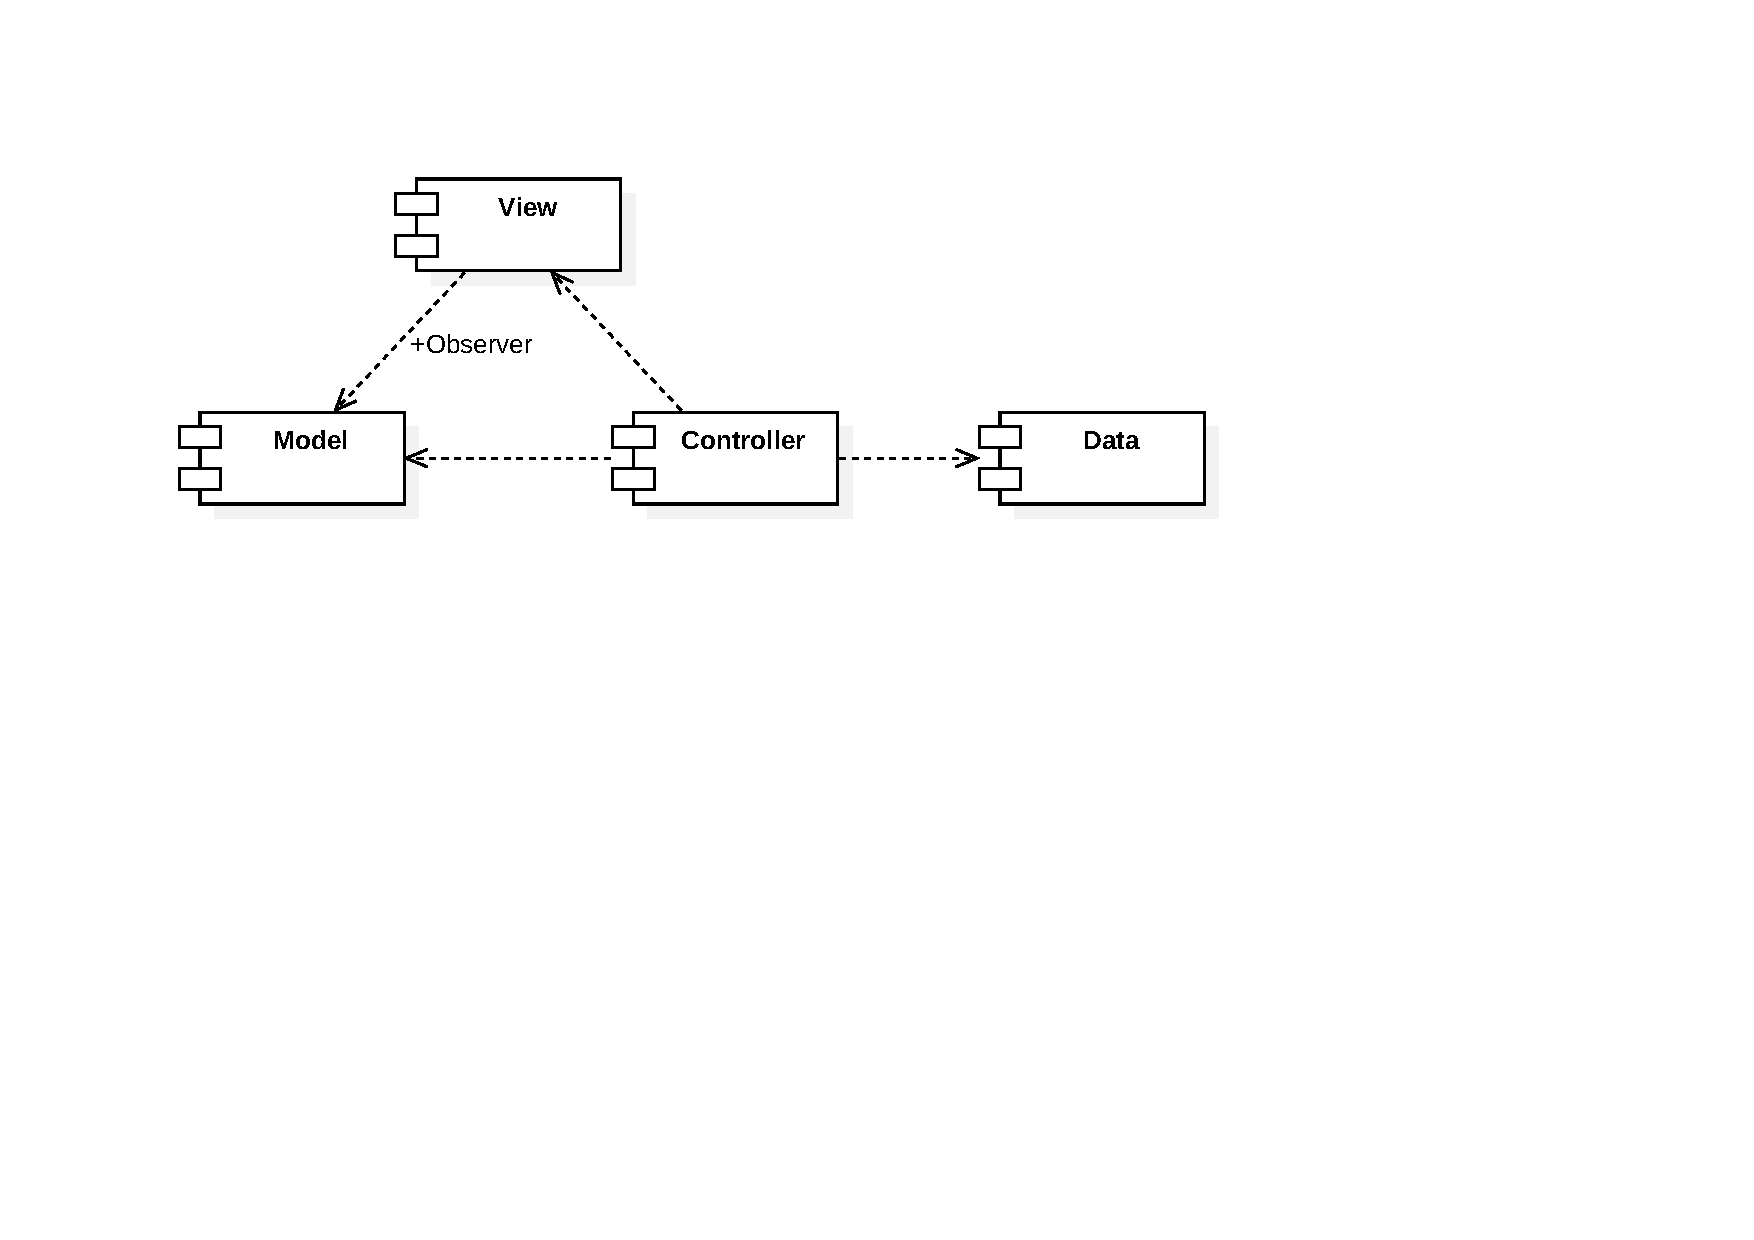
\includegraphics[trim=0 330 140 60,clip,width=\textwidth]{design/res/mvc}
    \end{center}
    \caption{MVC Architektur}
\end{figure}

Weil die Applikation stark durch das User Interface definiert ist, liegt eine Umsetzung mit dem MVC Pattern nahe.

\subsection{Variante C: Event Bus Architektur}
\begin{figure}[H]
    \begin{center}
    		% GFX Trim left bottom right top
        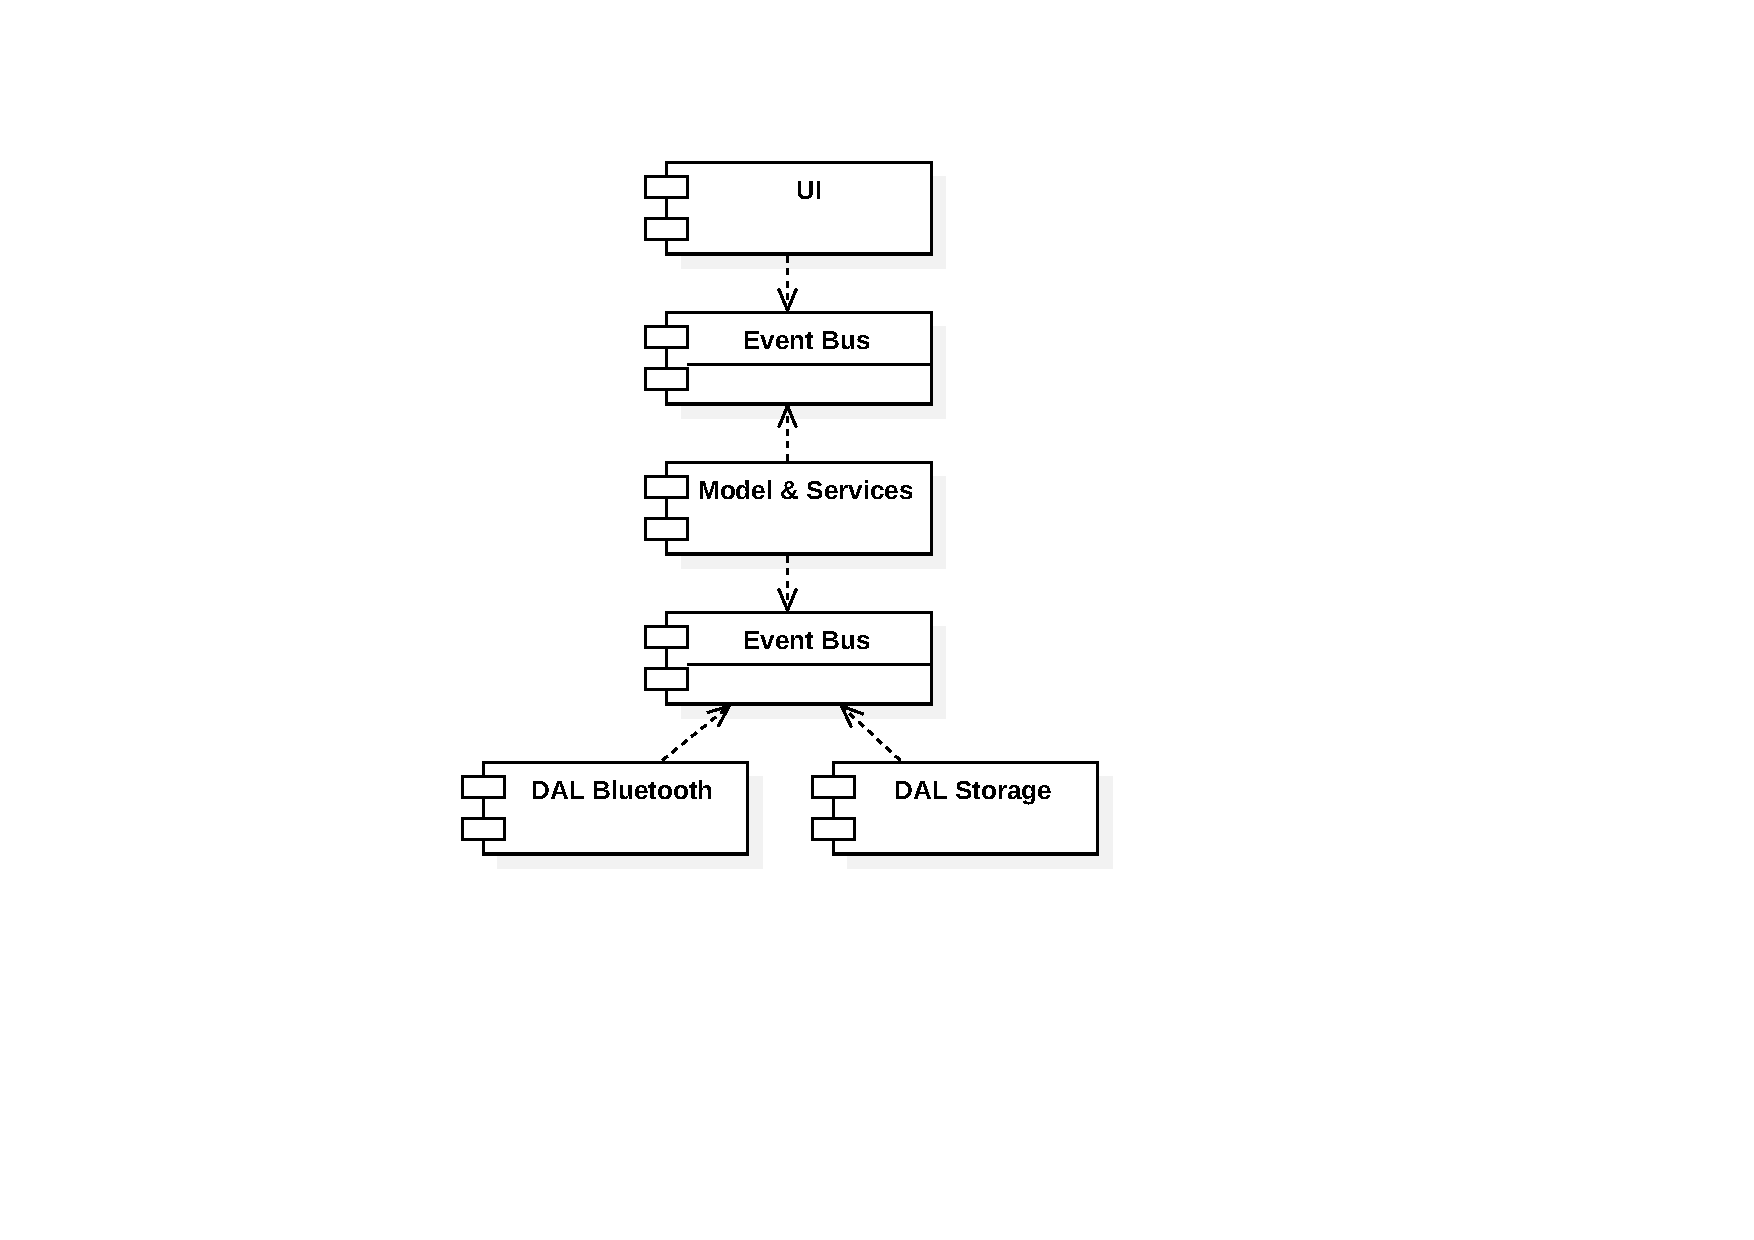
\includegraphics[trim=0 180 100 30,clip,width=\textwidth]{design/res/eventbus}
    \end{center}
    \caption{Event Bus Architektur}
\end{figure}

Mit einem Event Bus zwischen \ac{UI} und Model ist eine stärkere Entkopplung möglich\cite{fowler_event_collab}. Der Event Bus zwischen Model und \ac{DAL} ermöglicht mehrere Module wie Bluetooth und Storage.

\subsection{Bewertung der Architekturmöglichkeiten}

\begin{table}[H]
\begin{tabular}{|p{\textwidth{}/2}|p{\textwidth{}/2}|}
 \hline 
\multicolumn{2}{|c|}{\textbf{Variante A: Schichtenarchitektur}}\\ \hline 
Vorteile
\begin{enumerate}
\item Einfach verständlich, klassische Architektur
\item Separation of Concerns, Low Coupling, High Cohesion
\end{enumerate} & 
Nachteile
\begin{enumerate}
\item \ac{UI} Layer muss ganze Objekthierarchien beobachten
\item Kein einheitliches Parallelitätskonzept
\end{enumerate}
\\ \hline

\multicolumn{2}{|c|}{\textbf{Variante B: MVC Architektur}}\\ \hline 
Vorteile
\begin{enumerate}
\item Gute Entkopplung der View von der Logik
\item Reduktion von Navigationslogik
\end{enumerate} &
Nachteile
\begin{enumerate}
\item \ac{MVC} nur verwendbar in Kombination mit weiteren Patterns
\item Komplexe Observerstruktur zwischen View und Model
\item Kein einheitliches Parallelitätskonzept
\end{enumerate}
\\ \hline

\multicolumn{2}{|c|}{\textbf{Variante C: Event Bus Architektur}}\\ \hline 
Vorteile
\begin{enumerate}
\item Parallelität kann zentral von Bus synchronisiert werden
\item Einfachere Komponenten
\item Flache Observerstruktur im User Interface
\item Einfaches Hinzufügen von zusätzlichen Komponenten
\end{enumerate} &
Nachteile
\begin{enumerate}
\item Auf Grund flacher Hierarchie ist es leicht möglich Separation of Concerns zu verletzen.
\item Komplexere Interaktionslogik (Beispiel Message Chains)
\end{enumerate}
\\ \hline
\end{tabular}
\caption{Bewertung Architekturmöglichkeiten}
\end{table}

\subsubsection{Fazit}
Wir entscheiden uns für Variante C, denn sie ermöglicht uns die gewünschte konzeptionelle Erweiterbarkeit in Hinblick auf die \ac{FR} und \ac{NFR} die in Zukunft noch umgesetzt werden sollen. Zudem ermöglicht diese Architektur die Komplexität der Observer stark zu vereinfachen. Die stark asynchrone Kommunikation wird ideal unterstützt.

\section{Nebenläufigkeitskonzept}
\label{sec:Nebenläufigkeitskonzept}
Das Nebenläufigkeitskonzept bezieht sich auf Architektur Variante C \enquote{Event Bus}.

\subsection{Sicherstellen der Asynchronität}
Um sicherzustellen das alle Ereignisse asynchron verarbeitet werden, muss der Event Bus so konfiguriert werden dass er die Meldungsverarbeitung in einem eigenen Thread durchführt. Dies gilt auch für Meldungen die im \ac{UI}-Thread erzeugt werden. Damit ist sichergestellt das der \ac{UI}-Thread nicht blockiert.

\subsection{Synchronisierung mit \ac{UI}-Thread}
Zugriffe auf das User Interface dürfen nur vom UI-Thread durchgeführt werden. Dazu müssen die Subscriber dem Event Bus den gewünschten Ausführungsthread angeben können.

\subsection{Thread-Safety der Event Bus Subscriber}
Alle Subscribers müssen Sicherstellen (mit Ausnahme UI-Komponenten) dass von mehreren Threads aufgerufen werden können. Dazu werden klassische Java Monitors verwendet. Die Subscribers folgen dem "Run-to-completion" Prinzip.

\subsection{Restart von Activities}
Android kann zur Speicheroptimierung laufende Applikationen (im Hintergrund) ganz oder teilweise beenden. Öffnet der Benutzer die Applikation erneut muss sie ihren Zustand wiederherstellen. Dies erfordert eine Überprüfung dass die Instanzen im Application Context noch vorhanden sind. Gegebenenfalls müssen die Event Busse neu gestartet werden.

\nocite{*}
\bibliographystyle{IEEEtran}
\bibliography{Fluxron}


% \acs prints the longform the first time, after that the short
% using \ac always prints the shortform
   
\chapter*{List der Abkürzungen}\addcontentsline{toc}{chapter}{List of
Abbreviations}
\begin{acronym}[SPARC] % [] should contain the longest acronym
    \acro{API}{Application Programming Interface}
    \acro{CI}{Continuous Integration} 
	\acro{ECTS}{European Credit Transfer and Accumulation System}
	\acro{IDE}{Integrated Development Environment}
	\acro{JAR}{Java ARchive file}
	\acro{JVM}{Java Virtual Machine}
	\acro{HSR}{Hochschule für Technik Rapperswil}
	\acro{PDF}{Portable Document Format}
	\acro{TDD}{Test Driven Delevopment}
	\acro{UI}{User Interface}
	\acro{URL}{Uniform Resource Locator}
	\acro{VM}{Virtual Machine}
	\acro{XML}{Extensible Markup Language}
	\acro{LE}{Low Energy}
	\acro{FR}{Functional Requirement}
	\acro{NFR}{Non Functional Requirement}
\end{acronym}


\chapter{Anhang}
\label{chap:Anhang}

% Summary index document for the appendix
\appendix
\pagenumbering{Roman}

%Anhänge hier


\end{document}